\documentclass[a4paper,14pt]{extreport}
\usepackage[left=1.5cm,right=1.5cm,
    top=1.5cm,bottom=2cm,bindingoffset=0cm]{geometry}
\usepackage{scrextend}
\usepackage[T1,T2A]{fontenc}
\usepackage[utf8]{inputenc}
\usepackage[english,russian,ukrainian]{babel}
\usepackage{tabularx}
\usepackage{amssymb}
\linespread{1.5}
\usepackage{color}
\usepackage{amsmath}
\usepackage{mathrsfs}
\usepackage{listings}
\usepackage{graphicx}
\graphicspath{{./images/} }
\usepackage{lipsum}
\usepackage{xcolor}
\usepackage{hyperref}
\usepackage{tcolorbox}
\usepackage{tikz}
\usepackage[framemethod=TikZ]{mdframed}
\usepackage{wrapfig,boxedminipage,lipsum}
\mdfdefinestyle{MyFrame}{%
linecolor=blue,outerlinewidth=2pt,roundcorner=20pt,innertopmargin=\baselineskip,innerbottommargin=\baselineskip,innerrightmargin=20pt,innerleftmargin=20pt,backgroundcolor=gray!50!white}
 \usepackage{csvsimple}
 \usepackage{supertabular}
\usepackage{pdflscape}
\usepackage{fancyvrb}
%\usepackage{comment}
\usepackage{array,tabularx}
\usepackage{colortbl}

\usepackage{varwidth}
\tcbuselibrary{skins}
\usepackage{fancybox}


\usepackage{tikz}
\usepackage[framemethod=TikZ]{mdframed}
\usepackage{xcolor}
\usetikzlibrary{calc}
\makeatletter
\newlength{\mylength}
\xdef\CircleFactor{1.1}
\setlength\mylength{\dimexpr\f@size pt}
\newsavebox{\mybox}
\newcommand*\circled[2][draw=blue]{\savebox\mybox{\vbox{\vphantom{WL1/}#1}}\setlength\mylength{\dimexpr\CircleFactor\dimexpr\ht\mybox+\dp\mybox\relax\relax}\tikzset{mystyle/.style={circle,#1,minimum height={\mylength}}}
\tikz[baseline=(char.base)]
\node[mystyle] (char){#2};}
\makeatother

\definecolor{ggreen}{rgb}{0.4,1,0}
\definecolor{rred}{rgb}{1,0.1,0.1}
\definecolor{amber}{rgb}{1.0, 0.75, 0.0}
\definecolor{babyblue}{rgb}{0.54, 0.81, 0.94}
\definecolor{asparagus}{rgb}{0.53, 0.66, 0.42}
\definecolor{chartreuse}{rgb}{0.5, 1.0, 0.0}
\definecolor{darkorchid}{rgb}{0.6, 0.2, 0.8}

\usepackage{float}
\usepackage{wrapfig}
\usepackage{framed}
%for nice Code{
\lstdefinestyle{customc}{
  belowcaptionskip=1\baselineskip,
  breaklines=true,
  frame=L,
  xleftmargin=\parindent,
  language=C,
  showstringspaces=false,
  basicstyle=\small\ttfamily,
  keywordstyle=\bfseries\color{green!40!black},
  commentstyle=\itshape\color{purple!40!black},
  identifierstyle=\color{blue},
  stringstyle=\color{orange},
}
\lstset{escapechar=@,style=customc}
%}


\begin{document}
\pagecolor{white}

%----------------------------------------1
\newtcbox{\xmybox}[1][red]{on line, arc=7pt,colback=#1!10!white,colframe=#1!50!black, before upper={\rule[3pt]{0pt}{10pt}},boxrule=1pt,boxsep=0pt,left=6pt,right=6pt,top=2pt,bottom=2pt}


\begin{center}Bohdan Lyshchenko DP-82 Variant №4
\vspace{1cm}

\end{center}


\begin{center}VI. High permittivity microwave dielectrics \end{center}


Microwave (MW) dielectric ceramics have been used in mobile communications,
satellite television broadcasts, radar, Global Position System (GPS), Wireless Fidelity
(WiFi) and other modern communication systems as dielectric resonator (DR), filters,
duplexers and substrates, for almost half a century due to their high dielectric
permittivity $\left(\varepsilon_{\mathrm{r}}\right)$, high Qf $(\mathrm{Q} \sim \mathrm{MW}$ quality factor and $\mathrm{f} \sim$ resonant frequency) and
small temperature coefficient of resonant frequency (TCF). Since the first report of
MW dielectrics in the $\mathrm{BaO}-\mathrm{TiO}_{2}$ binary system,  ceramics with a range of $\varepsilon_{\mathrm{r}}$, high $\mathrm{Qf}$
and near-zero $\mathrm{TCF}$ such as the $\mathrm{Ba}(\mathrm{Zn}, \mathrm{Mg}, \mathrm{Co})_{1 / 3}(\mathrm{Nb}, \mathrm{Ta})_{2 / 3} \mathrm{O}_{3},(\mathrm{Sr}, \mathrm{Ca}) \mathrm{TiO}_{3}-\mathrm{LnAlO}_{3}$
$(\mathrm{Ln}=\mathrm{La}, \mathrm{Nd}, \mathrm{Sm}),(\mathrm{Zr}, \mathrm{Sn}) \mathrm{TiO}_{4}$ and $\mathrm{BaO}-\mathrm{Ln}_{2} \mathrm{O}_{3}-\mathrm{TiO}_{2}$ have been developed for use
from $300 \mathrm{MHz} \sim 40 \mathrm{GHz}$ by leading corporations such as Murata, Kyocera, EPCOS
and Trans-Tech.  In general, the roadmap for the development of MW dielectric
materials $^{2-4,6}$ may be separated into the following key target areas where there is a
technology pull from systems engineers and the absence suitable materials:
1) Expanding the range of $\varepsilon_{\mathrm{r}}$. Currently, most high Qf, zero TCF materials have
$20<\varepsilon_{\mathrm{r}}<50$ (base station resonators/antenna substrates) but there is a strong
technology pull for $5<\varepsilon_{\mathrm{r}}<20$ (higher bandwidth antenna substrates), $60<\varepsilon_{\mathrm{r}}$
$<70$ (base station resonators) and $\varepsilon_{\mathrm{r}}>120$ (ultra-small GPS antenna
substrates).\\

2) Low sintering temperature technology. The drive is to create a range of low
temperature co-fired ceramics (LTCC) compatible with Ag electrodes
(sintering temperature ~960$^{\circ}$) or ultra-low temperature co-fired ceramics
(ULTCC) compatible with Al as inner electrodes (sintering temperature < 660$^{\circ}$C). 

3) Ultrahigh Qf ceramics (>200,000 GHz).The focus here is to optimize Qf to 
achieve better selectivity to a specific frequency, critical for the transition from
4G to 5G technology in mobile telecommunications. 

4) Compositions based on low cost, abundant constituents. Here, the technology
is driven by scarcity, environmental concerns and geopolitical uncertainty
surrounding raw materials such as $\mathrm{Ta}_{2} \mathrm{O}_{5}, \mathrm{Nb}_{2} \mathrm{O}_{5}$, and $\mathrm{Ln}_{2} \mathrm{O}_{3}(\mathrm{Ln}=$ lanthanide).\\

Generically, MW dielectric ceramics are oxides, principallydue to the large ionic
polarizability of the $\mathrm{O}^{2} \text { -ion. } \text { Binary compounds, such as } \mathrm{MgO}, \mathrm{TiO}_{2}, \mathrm{Bi}_{2} \mathrm{O}_{3}, \mathrm{TeO}_{2} \text { , }$
$\mathrm{Al}_{2} \mathrm{O}_{3}$ and $\mathrm{CeO}_{2},{ }$ possess high Qf and in some cases useful $\varepsilon_{\mathrm{r}}$ but invariably have
large positive/negative TCF. Hence, ternary and higher compounds or compositesare
often explored to obtain temperature stable microwave dielectric ceramics with high
$\mathrm{Qf}^{1-15}$ The key to success in MW ceramicdevelopment is therefore in choosing,either
an adaptable crystal structure to form solid solutions or immiscible end members to
form composites that have no or limited interaction. Perovskite is the mostadaptable
crystal structure to form solid solution for $\mathrm{MW}$ ceramics $\left(\mathrm{ABO}_{3}\right)$ since a large number
of metallic elements may occupy the $\mathrm{A}$ and $\mathrm{B}$ sites in accordance with the
Goldschmidt tolerance factor, 
$\mathrm{t}=\left(\mathrm{R}_{\mathrm{A}}+\mathrm{R}_{\mathrm{B}}\right) / \sqrt{\left(\mathrm{R}_{\mathrm{B}}+\mathrm{R}_{\mathrm{O}}\right)}$
where $\mathrm{R}_{\mathrm{A}}, \mathrm{R}_{\mathrm{B}}$ and $\mathrm{R}_{\mathrm{O}}$ are the ionic radii of the $\mathrm{A}-\mathrm{B}$ - and $\mathrm{O}$ -site. Perovskitesdominate
medium and high permittivity commercial MW dielectrics in the range $25<\varepsilon_{\mathrm{r}}<60$
and $\varepsilon_{\mathrm{r}}>90^{8-13}$ Althoughefforts have been made to explore novel complex perovskite-structured microwave dielectrics with $\varepsilon_{r} \sim 65$, only limited progress has
been achieved with Qf $<12,500 \mathrm{GHz}$. ${ }^{28}$ Moreover, it is difficult to lower the sintering
temperatures of perovskites and related microwave dielectrics to meet the
requirements of LTCC technology. For example, commercial tungsten bronze
structured compounds achieve $70<\varepsilon_{\mathrm{r}}<90$ and $8,000<\mathrm{Qf}<12,000 \mathrm{GHz}$ when
sintered to full density. If the sintering temperature is lowered to $\sim 900^{\circ} \mathrm{C}$ by the
addition of glass, $\varepsilon_{\mathrm{r}}$ and Qf decrease to $\sim 65$ and $<6,000 \mathrm{GHz}$, respectively.  Despite
the great potential of LTCC technology and a substantial body of work in thescientific
literature, suppliers such as Dupont and Ferro offer only a limited range of
commercial LTCC materials. 








\newpage
\begin{figure}[h]
\center{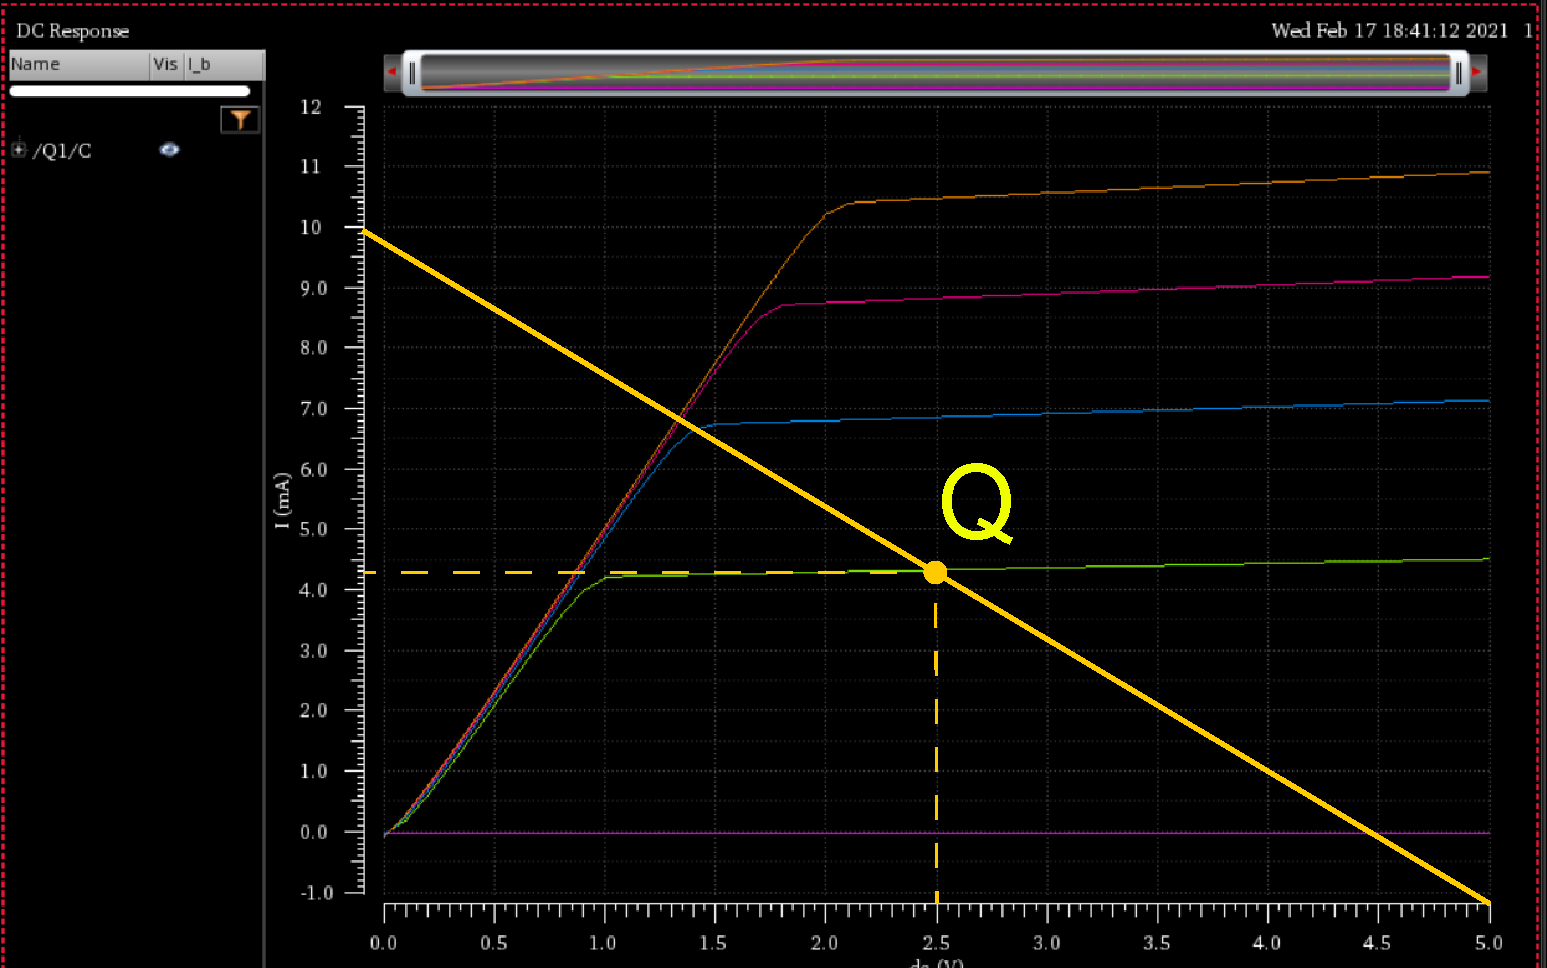
\includegraphics[width=0.6\linewidth]{1.png}}
\caption{XRD patterns of the $\mathrm{Bi}_{2}\left(\mathrm{Li}_{0.5} \mathrm{Ta}_{1.5}\right) \mathrm{O}_{7}+\mathrm{xBi}_{2} \mathrm{O}_{3}(\mathrm{x}=0,0.01$ and $0.02)$ ceramics
sintered at different temperatures and co-fired with $\mathrm{Bi}_{2}\left(\mathrm{Li}_{0.5} \mathrm{Ta}_{1.5}\right) \mathrm{O}_{7}+0.02 \mathrm{Bi}_{2} \mathrm{O}_{3}$ and
30 wt. \% silver powders}
\label{ris1}
\end{figure}

  Figure 1 shows the XRD patterns of $\mathrm{Bi}_{2}\left(\mathrm{Li}_{0.5} \mathrm{Ta}_{1.5}\right) \mathrm{O}_{7}+\mathrm{xBi}_{2} \mathrm{O}_{3}(\mathrm{x}=0,0.01$ and $0.02)$
ceramics sintered at different temperatures and co-fired with 30 wt. \% silver powder.
As reported by Muktha et al., $^{32}$ undoped $\mathrm{Bi}_{2}\left(\mathrm{Li}_{0.5} \mathrm{Ta}_{1.5}\right) \mathrm{O}_{7}$ crystalize in a variant of the
Aurivillius structure with a monoclinic, $\mathrm{C} 2 / \mathrm{c}$ space group. The diffraction peaksfrom
415141 -ICSD (Inorganic Crystal Structure Database) are also plotted in Figure 1. All
peaks were attributed to a single $\mathrm{Bi}_{2}\left(\mathrm{Li}_{0.5} \mathrm{Ta}_{1.5}\right) \mathrm{O}_{7}$ phase when sintered at their optimal
temperatures with no evidence of second phase, despite the addition of excess $\mathrm{Bi}_{2} \mathrm{O}_{3} .$
Although it is possible that excess $\mathrm{Bi}_{2} \mathrm{O}_{3}$ becomes incorporated in the lattice, Bi-rich
phases may also exsits but below the detectionlimit of the XRD equipment used
within this study. Results from Rietveld structural refinements are shown in Figure $\mathrm{S} 1$
of the supplementary material.











\end{document}